\documentclass[a4paper]{article}
\usepackage{geometry}
\geometry{a4paper,left=20mm,right=20mm, top=3cm, bottom=3cm} 
\usepackage[utf8]{inputenc}
\usepackage{graphicx}
\usepackage{hyperref}
\usepackage[ngerman]{babel}
\usepackage{float}
\usepackage{subcaption}
\usepackage{listings}
\usepackage{color}


\title{Validierungsbericht}
\date{\today{}, Passau}

\begin{document}
\begin{titlepage}
\vspace*{3cm}
\begin{center}
\textbf{\textsc{\LARGE Validierungsbericht}}

{\large \today}

\vspace{2cm}
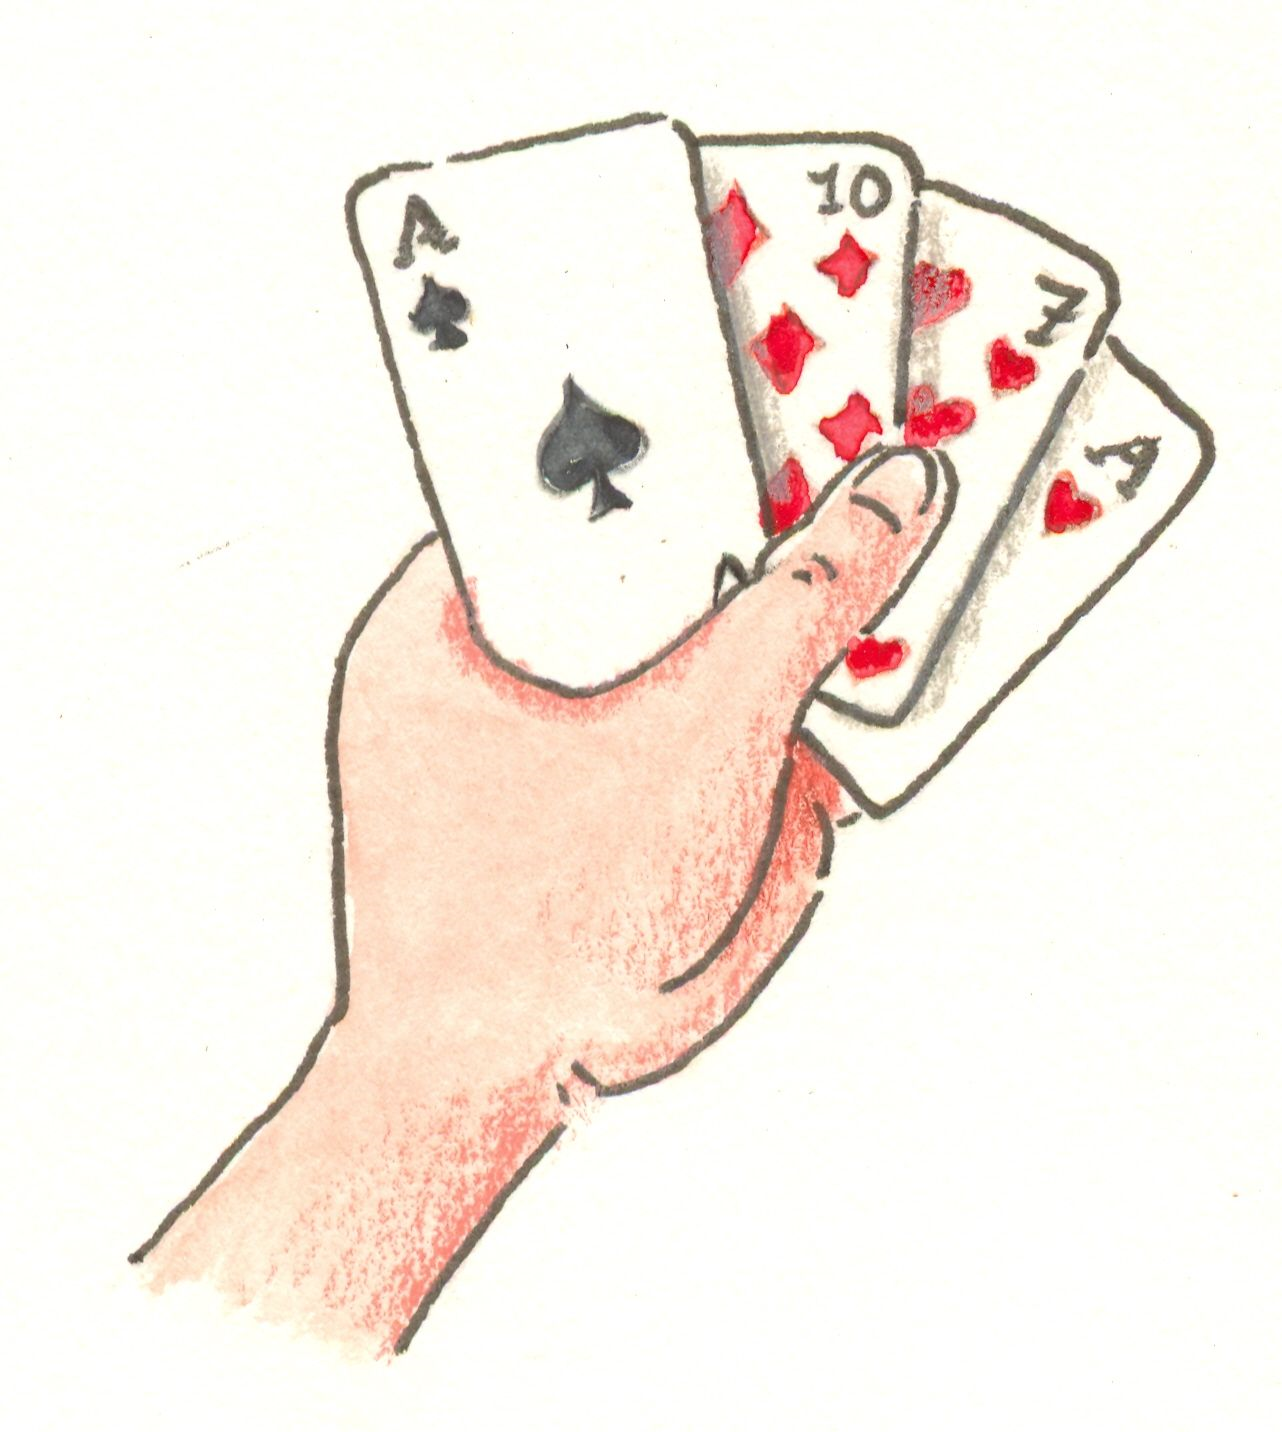
\includegraphics{kartenspiel}
\ \\
\ \\

\textbf{\textsc{\LARGE NET-WizHearts}}
\vspace{2cm}

\begin{tabular}{|c|c|c|}\hline
   Phase & Verantwortlicher & E-Mail \\ \hline\hline
   Pflichtenheft & Alina Meixl &  alina@meixl.de \\ \hline
   Entwurf & Viktoria Witka & witkaviktoria@freenet.de \\ \hline
   Spezifikation & Daniel Riedl & dariedl14@yahoo.de \\ \hline
   Implementation & Andreas Altenbuchner& a.andi007@gmail.com\\ \hline
   Validierung & Patrick Kubin & kubin@fim.uni-passau.de\\ \hline
   Präsentation & w& w\\ \hline
 \end{tabular}
\vspace{2cm}
\\
\end{center}
\end{titlepage}
\tableofcontents
\pagenumbering{arabic}
\hypersetup{pageanchor=true}

\newpage
 
\section{Einleitung}
Im folgenden Dokument werden alle Tests und ihre Ergebnisse aufgeführt, die im Rahmen der Testphase des Spiels NET-WizHearts abgeschlossen wurden, um die Funktionalitäten des Programms zu testen und deren Korrektheit zu bestätigen.

\section{Änderungen am Spiel}
\subsection{Änderungen zu vorherigen Phasen}
	\begin{itemize}
	\item{Kartenanzeige/Timer:} Um das Spiel benutzerfreundlicher zu gestalten wurde ein Timer eingefügt, der dafür sorgt, 		dass, wenn der letzte Spieler eines Umlaufes seine Karte ablegt, diese noch etwa eine Sekunde angezeigt werden, damit 		auch andere Mitspieler die zuletzt gelegte Karte erkennen können. 
	\item{Sortierung:} Die Karten der beiden Spiele werden nun sortiert um das Spiel übersichtlicher zu gestalten.
	\item{Spielende:} Es wurde eine Umfrage hinzugefügt, die es den Spielern erlaubt, nach dem Spielende direkt ein neues 		Spiel zu starten in der selben Zusammensetzung, wir zuvor, sofern jeder Spieler zustimmt.
	\item{Buttons:} Buttons, die nicht gedrückt werden können sind nun ausgegraut, statt einfach nur keine Reaktion 			hervorzurufen.
	\item{Rundenanzeige:} In dem Bereich, in welchem zuletzt die eigenen Informationen des Spieler angezeigt wurden, wird 		nun auch noch die Rundenzahl angezeigt.
	\end{itemize}
	
\subsection{Bereits bekannte und korrigierte Bugs}
Die Einstufung der Bugs erfolgt nach drei Kriterien:
\begin{itemize}
\item kritisch: \\
Der Fehler muss dringend behoben werden, da die Funktionen durch den Fehler stark beeinträchtigt werden.
\item wichtig: \\
Der Fehler sollte behoben werden, da Funktionen nicht einwandfrei genutzt werden können oder Verwirrungen für den Benutzer entstehen.
\item wünschenswert: \\
Es wäre gut, wenn der Fehler behoben würde. Da es sich jedoch um einen Schönheitsfehler handelt, ist dies nicht zwingend nötig, da die Funktionen des Programms nicht weiter eingeschränkt werden.
\end{itemize}
\ \\
\noindent
Es folgen aus der Implementierungsphase bekannte Bugs mit Ergebnis und Einstufung:
	\begin{itemize}
	\item \textbf{Hearts - Spielen der Karten:} Momentan wird beim Spielen von Hearts vom ServerRuleset keine Nachricht an 		alle ClientRulesets gesendet, wenn Herz gebrochen wird. Dadurch entsteht der Fehler, dass nur derjenige, der Herz 			gebrochen hat davon weiß und deshalb die anderen Mitspieler dennoch kein Herz spielen können. \\
	\textbf{Einstufung:} kritisch, da das Regelwerk nicht Fehlerfrei funktioniert hat. Dies macht Spielen unmöglich.\\
	\textbf{Ergebnis:} Der Fehler wurde behoben, die benötigte Nachricht wird jetzt gesendet. Dazu wurde eine neue RulesetMessage 'MsgBoolean' angelegt.\\
	
	\item \textbf{Abgelegte Karten:} Wir bei einem Umlauf im Spiel die letzte Karte gespielt, verschwinden alle Karten in 			diesem Moment. Die anderen Spieler haben so keine Möglichkeit, die zuletzt gespielte Karte zu erkennen. Dadurch ist es 			kaum möglich den Spielverlauf nachzuvollziehen. Deshalb sollen die Karten noch einige Sekunden angezeigt werden, bevor 		ein neuer Umlauf beginnt. \\
	\textbf{Einstufung:} wichtig, da es unter Umständen nötig ist, die gespielten gegnerischen Karten sehen zu können, um eine Strategie zu entwickeln. 
	\textbf{Ergebnis:} Der Fehler wurde behoben. Die Karten werden nun 1,2 Sekunden angezeigt.\\
	
	\item \textbf{Heartspunkte:} Beim Spiel Hearts wird bei den Informationen von jedem Spieler die Anzahl der gemachten 			Stiche statt der Punkte angezeigt. \\
	\textbf{Einstufung:} wichtig, da Informationen über die Punkte der gegnerischen Spieler ein strategisches Spielen ermöglichen, außerdem ist die Anzeige der eigenen Punkte von Nöten, um einen Spielüberblick zu behalten.\\
	\textbf{Ergebnis:} Der Fehler wurde behoben, die Anzeige ist jetzt richtig.

	\item \textbf{GUI Hearts:} Im Spiel Hearts werden rechts unten im Spielfenster Komponenten angezeigt, die das Spiel 			nicht benötigt, beispielsweise die Anzeige einer Trumpfkarte. \\
	\textbf{Einstufung:} wichtig, da ein Spieler womöglich durch funktionslose Felder auf dem Spielfeld verwirrt werden könnte.\\
	\textbf{Ergebnis:} Der Fehler wurde behoben. Unnötige Komponenten sind jetzt nicht mehr sichtbar.\\
	
	\item \textbf{Fehlermeldungen:} Einige Fehlermeldungen können noch optimiert werden. So enthält beispielsweise die 			Fehlermeldung bei der Eingabe eines falschen Passwortes einen Rechtschreibfehler im Wort 'incorrect'. \\
	\textbf{Einstufung:} wünschenswert, da alle Fehlermeldungen korrekt sind, jedoch Ausdrucks- und Rechtschreibfehler enthalten.\\
	\textbf{Ergebnis:} Der Fehler wurde behoben. Die Fehlermeldungen sind optimiert.\\
	
	\item \textbf{Kartenrückseite unter Linux:} Bild der Kartenrückseite wird unter Linux nicht sofort initialisiert, wenn das 			Spielfenster geöffnet wird, sondern erst beim Spielstart. \\
	\textbf{Einstufung:} wichtig, da es möglich war das Spiel fehlerfrei zu spielen, da die Kartenrückseiten nach der ersten Aktion erschienen, der Benutzer könnte jedoch von den zunächst leeren Feldern irritiert werden.\\
	\textbf{Ergebnis:} Der Fehler wurde behoben.\\
	
	\item \textbf{Spielende und Scorefenster:}  Das Spiel wird am Ende beendet, ohne dass ein Scorefenster angezeigt wird.\\
	\textbf{Einstufung:} kritisch, da keine Scores eingesehen werden können und auch kein Spiel neu gestartet werden kann. Es kann so kein Gewinner ermittelt werden. Es fehlt demnach eine vollständige Funktion des Spiels.\\
	\textbf{Ergebnis:} Der Fehler wurde behoben. Es wird nun ein Scorefenster mit dem Gewinner und den Punkten aller Mitspieler angezeigt. Des weiteren wird eine Umfrage gestartet, ob die Spieler eine weitere Runde spielen möchten. Bestätigen alle Spieler diese positiv, so wird ein neues Spiel gestartet. Ansonsten wird das Spiel aufgelöst und alle Spieler werden in die 		Lobby zurückgeleitet.\\
	
	\item \textbf{GUI Wizard:} Befindet man sich beim Spiel Wizard in der letzten Spielrunde, so gibt es keine Trumpfkarte oder 	Trumpffarbe mehr. Das Feld für diese beiden Anzeigen sollte also leer sein. Dies ist jedoch nicht der Fall, denn es wird 			immernoch die Trumpfkarte der vorherigen Runde angezeigt.\\
	\textbf{Einstufung:} wichtig, da das Spiel fehlerfrei gespielt werden konnte, jedoch die Karte sehr verwirrend für die Spieler ist und so falsche Vorhersagen getroffen werden.\\
	\textbf{Ergebnis:} Der Fehler wurde behoben. Das Kartenfeld ist in der letzten Runde leer.\\
	\end{itemize}
	
\subsection{Während der Validierung gefundene Bugs}
	Bugs, die während der Validierung gefunden wurden, werden an der entsprechenden Stelle detailliert ausgeführt.
	\begin{itemize}
	\item Gefunden durch Interaktive Spiel-Tests im Team
	\begin{itemize}
	\item{\textbf{Farbzwang-Bug Wizard:}} Wenn als erste Karte der Runde ein Narr gelegt wird und anschließend ein Zauberer, muss man die Farbe des Zauberers zugeben, obwohl man jede beliebiege Karte spielen können sollte.\\
	\textbf{Einstufung:} kritisch, da das Regelwerk falsche Aktionen fordert. Das Spiel funktioniert dadurch nicht mehr einwandfrei.\\
	\textbf{Ergebnis:} Der Fehler wurde behoben, indem kleine Änderungen in der isVaildMove-Methode der Klasse ClientWizard und ServerWizard vorgenommen wurden.
	\end{itemize}
	\item Gefunden durch JUnit-Testing
	\begin{itemize}
	\item{\textbf{Scorefenster-Bug:}} Wenn nach einem Spiel das Scorefenster geöffnet wird und der Spieler bei der Umfrage, ob ein neues Spiel gestartet werden soll auf 'nein' klickt, wird keine Aktion ausgeführt, da im Model kein ComObject für diesen Fall versendet wird. Gefunden wurde dieser Bug durch den ClientViewGamendTest.
	\textbf{Einstufung:} wichtig, da das Spiel auch auf das Klicken auf 'X' im Spielfeld beendet werden kann, jedoch die Umfrageoption nicht einwandfrei funktioniert.
	\textbf{Ergebnis:} Der Fehler wurde behoben. Das entsprechende ComObject wird versendet und das Spiel geschlossen. 
	
	\item{\textbf{Disconnect-Bug im Server:}} Im GameServer in den Methoden stand statt disconnectPlayer(player) nur player.closeConnection. Die Namen der Spieler, die das Spiel verließen, wurden deshalb nicht mehr frei gegeben.
Der Fehler wurde durch die GameServerCheatTests gefunden.\\
	\textbf{Einstufung:} kritisch, da ein Spieler nach dem Logout seinen Namen wieder benutzen können muss. Des weiteren würde die Liste mit den Spielernamen im Server immer länger werden und nie wieder weniger.\\
	\textbf{Ergebnis:} Der Fehler wurde behoben, die Namen werden wieder frei gegeben.
	\end{itemize}
\end{itemize}
 
	
\section{Plichtenheft Tests}
Die im Pflichtenheft beschriebenen Tests wurde alle ausgeführt und bestanden. Mit Ausnahme von Test /T240/. Hier wurde eine größere Änderung vorgenommen. Statt über eine Spieleinstellung und eine Pfadangabe ein neues Hintergrundbild einzufügen, muss des Benutzer das Bild nun in den Ordner 'Data' einfügen, es wird dann automatisch zur Auswahl hinzugefügt.\\
In folgenden Tests wurde der Text der Fehlermeldung verändert: /T025/, /T027/, /T029/, /T097/, /T280/, /T245/.  \\
In folgenden Tests wurde eine falsche Aktion durch die GUI unterbunden, statt eine Fehlermeldung auszugeben: /T092/, /T117/, /T182/, /T185/.  \\
In folgenden Tests wurde eine unnötige Nachricht vom Server im Chat weggelassen: /T170/, /T180/, /T228/, /T230/.\\
Es folgt eine genaue Beschreibung der Testfälle aus dem Pflichtenheft mit Testergebnis.
\begin{itemize}
	\item Login (keine Vorraussetzungen)
	\begin{itemize}
		
		\item /T020/ \textit{Verbindungsaufbau mit Server:} Mr. Blue gibt den Nickname 'MrBlue' und die Adresse des 			Servers ein (/F040/). Er verbindet sich mit dem Server und gelangt die Lobby (/F045/). \\
		Ergebnis: Der Test wurde bestanden.
		
		\item /T025/ \textit{Falsche Eingabe (Name):} Mr. Blue gibt keinen Namen ein, es kommt zu einer Fehlermeldung 				(/L290/ 'Kein Name angegeben'). \\
		Ergebnis: Der Test wurde bestanden. Die Fehlermeldung lautet 'Bitte gib einen Benutzernamen ein.'.
		
		\item /T027/ \textit{Falsche Eingabe (Name):} Nachdem Mr. Blue schon auf dem Server eingeloggt ist, 				versucht nun Mr. Bleau sich mit dem Nickname 'MrBlue' einzuloggen. Es wird eine Fehlermeldung angezeigt (/L290/ 			'Name wird bereits verwendet'). \\
		Ergebnis: Der Test wurde bestanden. Die Fehlermeldung lautet 'Login fehlgeschlagen. Der Benutzername ist bereits 			vergeben.'
		
		\item /T029/ \textit{Falsche Eingabe (IP):} Mr. Blue vertippt sich beim Eingeben der Serveradresse. Beim 				Loginversuch wird ein Fehler ausgegeben (/L290/  'Server konnte nicht gefunden werden'). \\
		Ergebnis: Der Test wurde bestanden. Die Fehlermeldung lautet 'Diese Adresse ist unbekannt.'
		
		\item /T030/ \textit{Auswahl der Sprache:} Mr. Blue wählt im Dropdown-Menü die Sprache 'English' aus (/F050W/), 			das Login-Fenster wird neu erstellt und es und alle folgenden Fenster sind nun in englischer Sprache. \\
		Ergebnis: Der Test wurde bestanden.
		
		\item /T035/ \textit{Beenden und wieder Einloggen:} Mr. Blue ist mit dem Namen 'MrBlue' eingeloggt. Er beendet das 		Spiel und der Nickname wird wieder freigegeben (/L380/). Er startet das Spiel noch einmal und loggt sich wieder mit 			'MrBlue' ein (/F045/). \\
		Ergebnis: Der Test wurde bestanden.
		
	\end{itemize}
	\item Lobby (Vorraussetzungen: /T020/) :
	\begin{itemize}
	
		\item /T040/ \textit{Spielerliste:} Der eigene Benutzername 'MrBlue' und die Benutzernamen aller anderen 					verbundenen Clients werden sofort in der Spielerliste angezeigt (/L100/). \\
		Ergebnis: Der Test wurde bestanden.
		
		\item /T050/ \textit{Serverliste:} Alle von Nutzern erstellten Spiele werden in der Spielliste angezeigt (/L110/). 			\\
		Ergebnis: Der Test wurde bestanden.
		
		\item /T060/ \textit{Chatnachricht senden:} Mr. Blue gibt die Nachricht 'Hallo Kartenwelt!' in das untere Textfeld ein 			und drückt die Entertaste (/F060/). Im oberen Textfeld wird die aktuellste Nachricht und alle bisher gesendeten 				Nachrichten angezeigt (/L115/). Mr. Pink ist auch in der Lobby, sieht die Nachricht von Mr. Blue (/L115/) und 				sendet die Nachricht 'Hallo MrBlue' (/F060/). Diese erscheint ebenfalls im Chat aller Spieler(/L115/). \\
		Ergebnis: Der Test wurde bestanden.
		
		\item /T080/ \textit{Spiel erstellen:} Mr. White erstellt ein Spiel und gelangt ins Erstellungsfenster (/F080/). \\
		Ergebnis: Der Test wurde bestanden.
		
		\item /T085/ \textit{Mehrere Spiele erstellen (Vorrausetzung: /T080/, /T110/):} Mr Pink erstellt ein weiteres Spiel 				und gelangt ins Erstellungsfenster (/F080/). Für alle eingeloggten Spieler sind nun beide Spiele sichtbar. \\
		Ergebnis: Der Test wurde bestanden.
		
		\item /T090/ \textit{Spiel beitreten:} Mr. Blue tritt dem bereits korrekt geöffneten und noch nicht vollen Spiel von Mr. 		White bei und gelangt ins Wartefenster (/F070/). \\
		Ergebnis: Der Test wurde bestanden. 
		
		\item /T092/ \textit{Fehler bei Spiel beitreten:} Mr. Brown hat kein Spiel aus der Liste ausgewählt. Er drückt den 				'Join'-Knopf und es wird eine Fehlermeldung angezeigt (/L290/ 'Kein Spiel ausgewählt'). \\
		Ergebnis: Der Test wurde bestanden. Es wird keine Fehlermeldung angezeigt, solange kein Spiel makiert wurde, ist 			der Button ausgegraut.
		
		\item /T095/ \textit{Passwortabfrage:} Das Spiel von Mr. White ist passwortgeschützt. Mr. Blue gibt 'youshouldtip' in 		das zugehörige Textfeld ein (/F140/) und drückt den 'Join'-Knopf, wodurch er zum Wartefenster weitergeleitet 			wird (/F142/).  \\
		Ergebnis: Der Test wurde bestanden.

		\item /T097/ \textit{Passwortabfrage(Abbruch):} Das Spiel von Mr. White ist passwortgeschützt. Mr. Blue kennt das 			Passwort nicht. Er gibt 'damn' in das Textfeld ein und drückt den 'Join'-Knopf. Eine Fehlermeldung erscheint (/L290/ 			'Falsches Passwort') und er bleibt in der Passwortabfrage. Er den 'Cancel'-Knopf und gelangt zurück in die 					Lobby (/F145/). \\
		Ergebnis: Der Test wurde bestanden. Es wird die Fehlermeldung ausgegeben 'Zutritt verweigert. Das Passwort ist 			inkorrekt.'
			  
	\end{itemize}
	\item Erstellungsfenster (Vorraussetzung: /T080/): 
	\begin{itemize}
	
		\item /T100/ \textit{Regelwerk auswählen:} Mr. White wählt 'Wizard' als Regelwerk aus (/F120/) und 				schaut sich dessen Logo an (/L120/), sowie eine kurze Beschreibung des Spiels, die erscheint, wenn er mit der Maus 			über das Logo fährt (/L122/). \\
		Ergebnis: Der Test wurde bestanden.
		
		\item /T105/ \textit{Regelwerk auswählen:} Mr. White wählt 'Hearts' als Regelwerk aus (/F120/) und 				schaut sich dessen Logo an (/L120/), sowie eine kurze Beschreibung des Spiels, die erscheint, wenn er mit der Maus 			über das Logo fährt (/L122/). \\
		Ergebnis: Der Test wurde bestanden.
		
		\item /T110/ \textit{Spiel erstellen:} Mr. White gibt 'NewHeist' als Spielname ein (/F122/). Er setzt einen Haken bei 			'Passwort' und gibt 'youshouldtip' als Passwort ein (/F130W/). Er drückt auf den 'Create'-Knopf, erstellt somit ein 				Spiel und wird zum Wartefenster weitergeleitet (/F126/). \\
		Ergebnis: Der Test wurde bestanden.
		
		\item /T115/ \textit{Spiel erstellen:} Mr. White gibt keinen Spielnamen an. Bei drücken des 'Create'-Knopfes wird ein 			Spiel mit dem Namen 'MrWhite`s Spiel' erstellt. \\
		Ergebnis: Der Test wurde bestanden.
		
		\item /T117/ \textit{Fehler bei Spiel erstellen:} Mr. White gibt 'NewHeist' als Spielname ein (/F122/). Er setzt einen 			Haken bei 'Passwort', aber vergisst ein Passwort einzugeben. Bei drücken des 'Create'-Knopfes wird eine 					Fehlermeldung angezeigt (/L290/ 'Kein Passwort gewählt'). \\
		Ergebnis: Der Test wurde bestanden. Solange kein Passwort in das Feld eingegeben wurde, obwohl der Haken 				gesetzt ist, kann der Erstellen-Button nicht gedrückt werden.
		
		\item /T120/ \textit{Erstellung abbrechen:} Mr. White erfährt, dass Mr. Pink schon in einem anderen Spiel ist und 				entschließt sich die Erstellung abzubrechen. Er drückt den 'Cancel'-Knopf und gelangt zurück in die Lobby		(/F124/). \\
		Ergebnis: Der Test wurde bestanden.
		
	\end{itemize}
	\item Wartefenster (Vorraussetzung: /T110/, /T090/)
	
	\begin{itemize}
		
		\item /T130/ \textit{Chat:} Mr. Pink und Mr. White befinden sich im Wartefenster des Spiels. Mr. Pink schreibt 			die Chatnachricht 'Hello Mr. White' und sie wird bei beidem im Chat angezeigt (/F160/). \\
		Ergebnis: Der Test wurde bestanden.
		
		\item /T170/ \textit{Verlassen:} Mr. Brown ist gerade dem Spiel beigetreten und verlässt es sofort wieder. Im Chat 			wird 'MrBrown ist dem Spiel beigetreten' angezeigt (/L270/). Er gelangt zurück in die Lobby (/T170/). Mr. White 			und Mr. Pink sehen den Namen 'MrBrown' kurz in der Spielerliste, bevor er wieder verschwindet. \\
		Ergebnis: Der Test wurde bestanden. Es wird keine Nachricht im Chat angezeigt, da diese unnötig ist.
		
		\item /T180/ \textit{Spieler entfernen:} Mr. Blue tritt dem Spiel bei. Mr. Pink hat das Spiel erstellt. Er ist somit 				Spielleiter und entschließt sich dazu Mr. Blue aus dem Spiel zu werfen (/F180/). Nach Drücken des 'Remove 				Player'-Knopfes gelangt Mr. Blue wieder in die Lobby. Mr. Blue erhält die Nachricht 'Sie wurden vom Spiel 				entfernt'. Im Chat wird angezeigt 'MrPink hat MrBlue vom Spiel entfernt'(/L270/). \\
		Ergebnis: Der Test wurde bestanden. Im Chat wird keine Nachricht angezeigt, da diese unnötig ist.
		
		\item /T182/ \textit{Fehler bei Spieler entfernen:} Mr. Pink ist Spielleiter. Er drückt den 'Remove Player'-				Knopf, hat aber keinen Spieler ausgewählt. Es wird eine Fehlermeldung angezeigt (/L290/ 'Kein Spieler ausgewählt'). 		\\
		Ergebnis: Der Test wurde bestanden. Es wird keine Fehlermeldung angezeigt, sondern der Button ist so lange 				ausgegraut, wie kein Spieler ausgewählt wurde. 
		
		\item /T185/ \textit{Fehler bei Starten des Spiels:} Mr. White ist allein im Wartefenster. Er drückt auf den 				'Start'-Knopf und es wird eine Fehlermeldung angezeigt (/L290/ 'Nicht genügend Spieler').
		Ergebnis: Der Test wurde bestanden. Es wird keine Fehlermeldung angezeigt, sondern der Button is so lange 				ausgegraut, bis genügend Spieler anwesend sind.
		
		\item /T190/ \textit{Spiel starten:} Mr. Brown und Mr. Orange treten dem Spiel bei. Es sind nun genug Spieler 				vorhanden, deshalb entschließt sich Mr. Pink dazu, das Spiel zu starten (/F200/). Alle Spieler gelangen ins 					Spielfenster, das Wartefenster wird geschlossen. \\
		Ergebnis: Der Test wurde bestanden.
		
		\item /T200/ \textit{Spiel auflösen:} Es dauert Mr. Pink zu lange, bis genug Spieler zusammenkommen, also verlässt 			er das Wartefenster. Da er der Spielleiter war, wird das Spiel aufgelöst und alle Spieler gelangen zurück 			zur Lobby (/F190/). \\
		Ergebnis: Der Test wurde bestanden.
		
	\end{itemize}
	\item Spielfenster Allgemein (Voraussetzung: /T190/)
	\begin{itemize}
	
		\item /T210/ \textit{Spielbeginn (Voraussetzung: /T100/):} Mr. Pink, Mr. White, Mr. Brown und Mr. Orange befinden 			sich im Spielfenster. Der Server teilt die Karten aus. Jeder sieht seine, ihm vom Server ausgeteilten 				Karten (/L190/) und die verdeckten Karten seiner Mitspieler (/L192/).   \\
		Ergebnis: Der Test wurde bestanden.
		
		\item /T220/ \textit{Zug: (Voraussetzung: /T210/)} Mr. Pink ist nicht am Zug, jedoch versucht er dennoch eine Karte 			zu spielen, was mit einem entsprechendem Dialog  unterbunden wird (/L290/). \\
		Ergebnis: Der Test wurde bestanden. Es wird die Fehlermeldung angezeigt 'Deine Aktion stimmt nicht mit der 				momentanen Spielphase überein.'.
		
		\item /T240/ \textit{Hintergrund ändern:} Mr. Pink klickt im Dropdown-Menü auf 'Einstellungen'. Ein Dialog mit einer 			Pfadabfrage öffnet sich. Mr. Pink gibt die Datei './neuerHintergrund.png' im Pfad an. Der Hintergrund des Spielfelds 			zeigt diese Bild an. \\
		Ergebnis: Der Test wurde bestanden. Der Spieler muss jedoch das Bild in den Ordner 'Data' einfügen. Im Spiel wird 			es automatisch zur Auswahl angezeigt, wenn der Spieler auf 'Hintergrund' drückt.
		
		\item /T270/ \textit{Spielende:} Mr. Orange spielt die letzte Karte des Spiels. Das Spiel ist zu Ende und der 					Server bestimmt den Gewinner. Mr. Orange bekommt eine Zusammenfassung angezeigt, die ihn als Sieger 				erklärt und seine Punkte anzeigt(/L250/). Alle anderen Spieler erhalten ebenfalls eine Zusammenstellung ihrer 				Leistung (/L250/). \\
		Ergebnis: Der Test wurde bestanden. Jeder Spieler bekommt eine Übersicht auf der eingesehen werden kann, 				welcher Spieler gewonnen hat und wie viele Punkte jeder einzelne Spieler erreicht hat.
		
		\item /T280/ \textit{Spielabbruch: (Voraussetzung /T190/)} Es läuft für Mr. Pink nicht sonderlich gut und er 					entschließt sich, es sein zu lassen, weshalb er das Spiel durch einen Klick auf 'schließen' beendet und sich 					anschließend in der Lobby wiederfindet (/F210/). Mr. White, Mr. Brown und Mr. Orange werden über das 				Verlassen des Spielers 'Mr. Pink' durch eine Fehlermeldung informiert (/L290/) und werden ebenfalls in die 					Lobby zurückgeworfen. \\
		Ergebnis: Der Test wurde bestanden. Die anderen Spieler erhalten die Fehlermeldung 'Das Spiel wurde aufgelöst'.
	
		\item /T300/ \textit{Chat:} Mr. Pink, Mr. White, Mr. Brown und Mr. Orange befinden sich im Spielfenster. Mr. Orange 			schreibt die Chatnachricht 'Hallo zusammen!' (/F220/) und sie wird bei allen im Chat angezeigt (/L260/). \\
		Ergebnis: Der Test wurde bestanden.
	
		\item /T310/ \textit{Chat:} Mr. Pink, Mr. White, Mr. Brown und Mr. Orange befinden sich im Spielfenster. Mr. Orange 			versucht eine leere Nachricht im Chatfenster abzusetzen, die Nachricht wird nicht gesendet und erscheint auch 				nicht in seinem Chat. \\
		Ergebnis: Der Test wurde bestanden.
		
		\item /T320/ \textit{Neue Runde:} Das Spiel wurde fertig gespielt. Jeder Mitspieler erhält eine Abfrage ('Nochmal 				spielen?') (/L275W/). Jeder Spieler stimmt mit 'Ja'. Es wird ein neues Spiel gestartet (/F200/). \\
		Ergebnis: Der Test wurde bestanden. Die Abfrage befindet sich im selben Fenster, wie Übersicht am Ende eines 				Spiels.
		
		
	\end{itemize}\item Spielfenster Wizard
	\begin{itemize}
		\item /T228/ \textit{Rundenbeginn: (Vorraussetzung: /T210/)} Der Server dreht die oberste Karte auf dem 				Aufnahmestapel (/L195/) automatisch um und sagt dadurch die Trumpffarbe (ausgenommen einen Zauberer) an. Im 			Chat erscheint eine Spielnachricht des Servers (/L270/). \\
		Ergebnis: Der Test wurde bestanden. Es wird keine Nachricht im Chat angezeigt, da diese unnötig ist.

		\item /T230/ \textit{Stiche ansagen: (Voraussetzung: /T228/)} Nach längerem Spiel wird einer der 4 Zauberer vom 			Server beim Kartengeben aufgedeckt und da Mr. Pink an der Reihe ist, erscheint ein Auswahlfenster. Mr. Pink 			wählt die Trumpffarbe. (/F360/) Über den Spielchat erhalten alle Spieler Auskunft über den Vorgang (/L270/) und 				sehen die angesagte Farbe. \\
		Ergebnis: Der Test wurde bestanden. Es wird keine Chatnachricht gesendet, sondern die Farbe wird in dem 				zusätzlichen Feld für die Trumpffarbe angezeigt.
	
		\item /T240/ \textit{Stiche ansagen: (Voraussetzung: /T228/ oder /T230/)} Nachdem eine Trumpffarbe angesagt 				wurde erscheint ein Fenster, indem jeder Spieler die Anzahl seiner Stiche tippen kann. Mr. Brown glaubt 4 Stiche 				machen zu können und gibt die Zahl ein (/F370/). Auch die anderen Spieler geben ihre Tipps ab und sehen die 				prognostizierten Stiche der anderen.(/L196/). \\
		Ergebnis: Der Test wurde bestanden.
		
		\item /T245/ \textit{Stiche ansagen: (Voraussetzung: /T228/ oder /T230/)} Nachdem eine Trumpffarbe angesagt 				wurde erscheint ein Fenster, indem jeder Spieler die Anzahl seiner Stiche tippen kann. Mr. Orange gibt 'zehn' in das 			Feld ein. Es wird eine Fehlermeldung angezeigt (/L290/ 'Bitte geben sie eine Zahl ein'). \\
		Ergebnis: Der Test wurde bestanden. Es wird die Fehlermeldung 'Diese Zahl ist nicht erlaubt.' angezeigt.
		
		\item /T260/ \textit{Rundenende:} Mr. Pink spielt die letzte Karte der Runde. Es erscheint eine kurze 					Zusammenfassung, wie viele Stiche er gemacht hat, wie viele er getippt hat und erhält seinen aktuellen Punkestand 			sowie den der anderen Mitspieler in einem separatem Fenster angezeigt (/L250/). \\
		Ergebnis: Der Test wurde bestanden. Jeder Spieler hat eine Feld, in dem die oben genannten Informationen 				angezeigt werden. 
					
	\end{itemize}
	
	\item Spielfenster Hearts
	\begin{itemize}
	
		\item /T290/ \textit{Spielbeginn Hearts: (Voraussetzung /T105/)} Mr. Pink, Mr. White, Mr. Orange und Mr. Brown 				befinden sich im Spielfenster. Das Spiel beginnt und ein Fenster erscheint bei allen Spielern in dem 3 Karten 				ausgewählt werden müssen. Mr. White wählt 3 Karten aus und bestätigt seine Auswahl (/F260/). Nachdem Mr. 				Orange ebenfalls 3 Karten zur Weitergabe ausgewählt hat erhält diese Mr. White. Mr. Pink erhält die 3 Karten von 			Mr. White und  Mr. Orange erhält die Karten von Mr. Pink. \\
		Ergebnis: Der Test wurde bestanden.

		\item /T295/ \textit{Spielbeginn Hearts: (Voraussetzung /T105/)} Mr. Pink, Mr. White, Mr. Orange und Mr. Brown 				befinden sich im Spielfenster. Das Spiel beginnt und ein Fenster erscheint bei allen Spielern, in dem 3 Karten 				ausgewählt werden müssen. Mr. White nur 2 Karten aus und bestätigt seine Auswahl (/F260/). Es erscheint ein 				Dialog der ihn auffordert 3 Karten auszuwählen(/L290/). \\
		Ergebnis: Der Test wurde bestanden. Die Fehlermeldung lautet 'Du kannst diese Karten nicht tauschen.'.

		\item /T330/ \textit{Zug: (Vorausetzung /T210/)} Mr. Pink versucht eine ungültige Karte zuzugeben. Das Spiel 				erkennt den Regelverstoß und zeigt dies über einen Dialog an (/L290/). \\
		Ergebnis: Der Test wurde bestanden. Die Fehlermeldung lautet 'Der Zug ist nicht gültig!'.
		
	\end{itemize}
\end{itemize}

\section{Line- und Branch-Coverage}
	\subsection{View}
	Die View wurde in erster Linie durch einen interaktiven Test getestet. Auch über JUnit-Tests gibt es für die View Ergebnisse, die jedoch nicht ausreichend sind, da nicht versucht wurde eine möglichst hohe Abdeckung zu erreichen.
Der Interaktive Test ist somit der aussagekräftigere Test und wird im Anschluss ebenfalls zu den Ergebnissen der JUnit-Tests aus den anderen Paketen gerechnet.
	\subsubsection{Interaktiver Test}
	\begin{itemize}
	\item Betrachtete Testfälle:
	/T020/, /T025/, /T027/, /T029/, /T030/, /T040/, /T050/, /T060/, /T080/, /T085/, /T090/, /T095/, /T097/, /T100/, /T105/, 		/T110/, /T115/, /T120/, /T130/, /T170/, /T180/, /T190/, /T200/, /T210/, /T220/, /T240/, /T280/, /T300/, /T310/, /T228/, 		W/T240/, /T245/,  /T250/, /T290/, /T295/, /T330/  \\
	\item Nicht betrachtete Testfälle: \\
	\begin{itemize}
	\item Fehlermeldung durch ausgegrauten Button ersetzt: /T092/, /T117/, /T182/, /T185/. \\
	\item Testfall, der das Programm beenden würden und somit die Coverage-Aufzeichnung unterbrechen würde: /T035/. \\
	\item Vom Zufall abhängig (eigentlich deswegen auch kein Testfall): /T230/. \\
	\item Setzen Ende des Spiels vorraus, Zeitaufwand zu hoch: /T270/, /T320/, /T260/. \\
	\end{itemize}
	\end{itemize}
	
	\noindent
\begin{tabular}{|l|r|r|}
\hline
Classes in this Package & \multicolumn{1}{l|}{Line Coverage in \%} & \multicolumn{1}{l|}{Branch Coverage in \%} \\ \hline
GamePanel & 96,5 & 93,5 \\ \hline
ScoreWindow & 64,1 & 31,2 \\ \hline
ChooseItem & 65,1 & 33,3 \\ \hline
Game & 96,6 & 78,6 \\ \hline
ViewCard & 89,6 & 83,3 \\ \hline
CreateGame & 86,2 & 58,6 \\ \hline
Lobby & 93,9 & 73,3 \\ \hline
ChooseCards & 91,9 & 66,7 \\ \hline
Warning & 82,2 & 40 \\ \hline
DiscardPile & 70,6 & \multicolumn{1}{l|}{} \\ \hline
TrumpColour & 78,3 & 57,1 \\ \hline
GameLobby & 98,5 & 87,5 \\ \hline
InputNumber & 93,5 & 75 \\ \hline
Language & 100 & \multicolumn{1}{l|}{} \\ \hline
DrawDeck & 83,3 & \multicolumn{1}{l|}{} \\ \hline
OtherPlayer & 96,9 & 100 \\ \hline
Login & 92,9 & 66,7 \\ \hline
Password & 97 & 71,4 \\ \hline
OwnHand & 100 & 100 \\ \hline
OwnOtherData & 100 & 100 \\ \hline
 & \multicolumn{1}{l|}{} & \multicolumn{1}{l|}{} \\ \hline
View Gesamt & 90,6 & 72,5 \\ \hline
\end{tabular}

 	Resultate vom interaktiven Test bei restlichen Paketen: \\\\
 	\noindent
 	\begin{tabular}{|l|r|l|}\hline
 	Klasse & Line Coverage in \% & Branch Coverage in \% \\ \hline \hline
Ruleset & 5,4 & 3.7 \\ \hline
Server & \multicolumn{1}{l|}{-} & - \\ \hline
Client & 34,1 & \multicolumn{1}{r|}{37,9} \\ \hline
ComObjects & 36,8 &  \\ \hline
 & \multicolumn{1}{l|}{} &  \\ \hline
Gesamt & 22,2 & \multicolumn{1}{r|}{17,2} \\ \hline
\end{tabular}

\subsubsection{JUnitTest-Ergebnisse}
Die Ergebnisse ergeben sich aus wenigen Tests, die eien View öffnen. Sie können nicht als aussagegräftige Ergebnisse gezählt werden. Der Interaktive Test beschreibt die Ergebnisse genauer.

\noindent
\begin{tabular}{|l|l|l|l|}
\hline
Package & \# Classes & Line Coverage & Branch Coverage \\ \hline
Client.View & \multicolumn{1}{r|}{63} & \multicolumn{1}{r|}{59,00\%} & \multicolumn{1}{r|}{42,00\%} \\ \hline
\end{tabular}

\ \\

\noindent
\begin{tabular}{|l|r|l|}
\hline
Classes in this Package & \multicolumn{1}{l|}{Line Coverage} & Branch Coverage \\ \hline
ChooseCards & 78,00\% & \multicolumn{1}{r|}{66,00\%} \\ \hline
ChooseCards\$1 & 0,00\% & N/A \\ \hline
ChooseCards\$2 & 0,00\% & N/A \\ \hline
ChooseCards\$3 & 0,00\% & N/A \\ \hline
ChooseCards\$4 & 100,00\% & N/A \\ \hline
ChooseCards\$CardMouseListener & 0,00\% & \multicolumn{1}{r|}{0,00\%} \\ \hline
ChooseItem & 69,00\% & \multicolumn{1}{r|}{50,00\%} \\ \hline
ChooseItem\$1 & 0,00\% & N/A \\ \hline
CreateGame & 60,00\% & \multicolumn{1}{r|}{44,00\%} \\ \hline
CreateGame\$1 & 0,00\% & \multicolumn{1}{r|}{0,00\%} \\ \hline
CreateGame\$2 & 0,00\% & N/A \\ \hline
CreateGame\$3 & 100,00\% & N/A \\ \hline
CreateGame\$LeaveButtonListener & 0,00\% & N/A \\ \hline
CreateGame\$MouseOverListener & 0,00\% & N/A \\ \hline
CreateGame\$PWCheckedListener & 0,00\% & \multicolumn{1}{r|}{0,00\%} \\ \hline
CreateGame\$PWEmptyListener & 0,00\% & \multicolumn{1}{r|}{0,00\%} \\ \hline
CreateGame\$RulesetSelectionListener & 100,00\% & N/A \\ \hline
DiscardPile & 70,00\% & N/A \\ \hline
DrawDeck & 83,00\% & N/A \\ \hline
Game & 70,00\% & \multicolumn{1}{r|}{51,00\%} \\ \hline
Game\$1 & 64,00\% & \multicolumn{1}{r|}{60,00\%} \\ \hline
Game\$2 & 100,00\% & N/A \\ \hline
Game\$3 & 0,00\% & N/A \\ \hline
Game\$4 & 0,00\% & N/A \\ \hline
Game\$5 & 40,00\% & \multicolumn{1}{r|}{50,00\%} \\ \hline
Game\$6 & 0,00\% & N/A \\ \hline
Game\$bgMenuAction & 0,00\% & N/A \\ \hline
Game\$cardsMenuAction & 0,00\% & N/A \\ \hline
GameLobby & 71,00\% & \multicolumn{1}{r|}{44,00\%} \\ \hline
GameLobby\$1 & 91,00\% & \multicolumn{1}{r|}{66,00\%} \\ \hline
GameLobby\$2 & 71,00\% & \multicolumn{1}{r|}{50,00\%} \\ \hline
GameLobby\$3 & 0,00\% & N/A \\ \hline
GameLobby\$PlayerSelectedListener & 0,00\% & \multicolumn{1}{r|}{0,00\%} \\ \hline
GamePanel & 55,00\% & \multicolumn{1}{r|}{41,00\%} \\ \hline
InputNumber & 67,00\% & \multicolumn{1}{r|}{66,00\%} \\ \hline
InputNumber\$1 & 0,00\% & N/A \\ \hline
InputNumber\$2 & 0,00\% & N/A \\ \hline
Language & 100,00\% & N/A \\ \hline
Lobby & 59,00\% & \multicolumn{1}{r|}{28,00\%} \\ \hline
Lobby\$1 & 0,00\% & N/A \\ \hline
Lobby\$2 & 100,00\% & N/A \\ \hline
Lobby\$3 & 0,00\% & N/A \\ \hline
Lobby\$4 & 100,00\% & N/A \\ \hline
Lobby\$5 & 0,00\% & N/A \\ \hline
Lobby\$GameSelectedListener & 0,00\% & \multicolumn{1}{r|}{0,00\%} \\ \hline
\end{tabular}

\noindent
\begin{tabular}{|l|r|l|}
\hline
Classes in this Package & \multicolumn{1}{l|}{Line Coverage} & Branch Coverage \\ \hline
Login & 73,00\% & \multicolumn{1}{r|}{63,00\%} \\ \hline
Login\$1 & 0,00\% & N/A \\ \hline
Login\$NameLengthListener & 0,00\% & \multicolumn{1}{r|}{0,00\%} \\ \hline
Login\$NameLengthListener\$1 & 0,00\% & N/A \\ \hline
OtherPlayer & 62,00\% & \multicolumn{1}{r|}{50,00\%} \\ \hline
OwnHand & 92,00\% & \multicolumn{1}{r|}{100,00\%} \\ \hline
OwnOtherData & 66,00\% & \multicolumn{1}{r|}{50,00\%} \\ \hline
Password & 58,00\% & \multicolumn{1}{r|}{36,00\%} \\ \hline
Password\$1 & 0,00\% & N/A \\ \hline
Password\$LeaveButtonListener & 0,00\% & N/A \\ \hline
ScoreWindow & 66,00\% & \multicolumn{1}{r|}{41,00\%} \\ \hline
ScoreWindow\$1 & 80,00\% & \multicolumn{1}{r|}{50,00\%} \\ \hline
ScoreWindow\$2 & 100,00\% & N/A \\ \hline
TrumpColour & 16,00\% & \multicolumn{1}{r|}{0,00\%} \\ \hline
ViewCard & 43,00\% & \multicolumn{1}{r|}{16,00\%} \\ \hline
Warning & 79,00\% & \multicolumn{1}{r|}{60,00\%} \\ \hline
Warning\$1 & 0,00\% & N/A \\ \hline
Warning\$CloseListener & 0,00\% & \multicolumn{1}{r|}{0,00\%} \\ \hline
\end{tabular}

	
	\subsection{Client}
	
	\noindent
	\begin{tabular}{|l|l|l|l|} \hline
	Package & \ Classes & Line Coverage & Branch Coverage \\ \hline \hline
	Client & \multicolumn{1}{r|}{32} & \multicolumn{1}{r|}{56,00\%} & \multicolumn{1}{r|}{56,00\%} \\ \hline
	\end{tabular}

	\noindent	
\begin{tabular}{|l|r|l|}
\hline
Classes in this Package & \multicolumn{1}{l|}{Line Coverage} & Branch Coverage \\ \hline \hline
ClientController & 79,00\% & \multicolumn{1}{r|}{50,00\%} \\ \hline
ClientController\$CardMouseListener & 0,00\% & \multicolumn{1}{r|}{0,00\%} \\ \hline
ClientController\$ChatListenerGame & 0,00\% & \multicolumn{1}{r|}{0,00\%} \\ \hline
ClientController\$ChatListenerGameLobby & 0,00\% & \multicolumn{1}{r|}{0,00\%} \\ \hline
ClientController\$ChatListenerLobby & 0,00\% & \multicolumn{1}{r|}{0,00\%} \\ \hline
ClientController\$ConnectButtonListener & 0,00\% & N/A \\ \hline
ClientController\$CreateButtonListener & 0,00\% & \multicolumn{1}{r|}{0,00\%} \\ \hline
ClientController\$GameCloseListener & 0,00\% & N/A \\ \hline
ClientController\$GameLobbyCloseListener & 12,00\% & N/A \\ \hline
ClientController\$HostButtonListener & 0,00\% & N/A \\ \hline
ClientController\$JoinButtonListenerLobby & 0,00\% & \multicolumn{1}{r|}{0,00\%} \\ \hline
ClientController\$JoinButtonListenerPassword & 0,00\% & N/A \\ \hline
ClientController\$KickPlayerButtonListener & 0,00\% & N/A \\ \hline
ClientController\$LanguageSelectionListener & 0,00\% & N/A \\ \hline
ClientController\$LeaveButtonListenerGameLobby & 0,00\% & N/A \\ \hline
ClientController\$LeaveButtonListenerLobby & 0,00\% & N/A \\ \hline
ClientController\$LeaveButtonListenerPassword & 0,00\% & N/A \\ \hline
ClientController\$LeaveButtonListenerScoreWindow & 0,00\% & N/A \\ \hline
ClientController\$LobbyCloseListener & 12,00\% & N/A \\ \hline
ClientController\$OKButtonListenerChooseCards & 0,00\% & N/A \\ \hline
ClientController\$OKButtonListenerChooseColour & 0,00\% & N/A \\ \hline
ClientController\$OKButtonListenerInputNumber & 0,00\% & \multicolumn{1}{r|}{0,00\%} \\ \hline
ClientController\$OKButtonListenerWarning & 0,00\% & \multicolumn{1}{r|}{0,00\%} \\ \hline
ClientController\$PlayAgainButtonListenerScoreWindow & 0,00\% & N/A \\ \hline
ClientController\$StartGameButtonListener & 0,00\% & N/A \\ \hline
ClientMain & 0,00\% & N/A \\ \hline
ClientMain\$1 & 0,00\% & N/A \\ \hline
ClientModel & 89,00\% & \multicolumn{1}{r|}{81,00\%} \\ \hline
ClientState & 93,00\% & N/A \\ \hline
LanguageInterpreter & 25,00\% & \multicolumn{1}{r|}{26,00\%} \\ \hline
MessageListenerThread & 0,00\% & \multicolumn{1}{r|}{0,00\%} \\ \hline
ViewNotification & 100,00\% & N/A \\ \hline
\end{tabular}


	\subsection{Server}

	\noindent	
\begin{tabular}{|l|l|l|l|}
\hline
Package & \# Classes & Line Coverage & Branch Coverage \\ \hline \hline
Server & \multicolumn{1}{r|}{8} & \multicolumn{1}{r|}{76,00\%} & \multicolumn{1}{r|}{75,00\%} \\ \hline
\end{tabular}

\noindent
\begin{tabular}{|l|r|r|}
\hline
Classes in this Package & \multicolumn{1}{l|}{Line Coverage} & \multicolumn{1}{l|}{Branch Coverage} \\ \hline
GameServer & 86,00\% & 79,00\% \\ \hline
GameServerRepresentation & N/A & \multicolumn{1}{l|}{N/A} \\ \hline
LobbyServer & 90,00\% & 84,00\% \\ \hline
LoginServer & 91,00\% & 75,00\% \\ \hline
LoginServer\$ClientListenerThread & 50,00\% & 50,00\% \\ \hline
Player & 13,00\% & 0,00\% \\ \hline
Server & 83,00\% & 80,00\% \\ \hline
ServerMain & 0,00\% & 0,00\% \\ \hline
\end{tabular}


 	
	\subsection{Ruleset}
	
\noindent	
\begin{tabular}{|l|l|l|l|}
\hline
Package & \# Classes & Line Coverage & Branch Coverage \\ \hline \hline
Ruleset & \multicolumn{1}{r|}{24} & \multicolumn{1}{r|}{89,00\%} & \multicolumn{1}{r|}{84,00\%} \\ \hline
\end{tabular}

\noindent
\begin{tabular}{|l|r|l|}
\hline
Classes in this Package & \multicolumn{1}{l|}{Line Coverage} & Branch Coverage \\ \hline \hline
Card & N/A & N/A \\ \hline 
CardComparator & 99,00\% & \multicolumn{1}{r|}{87,00\%} \\ \hline
ClientHearts & 100,00\% & \multicolumn{1}{r|}{100,00\%} \\ \hline
ClientRuleset & 65,00\% & \multicolumn{1}{r|}{54,00\%} \\ \hline
ClientWizard & 100,00\% & \multicolumn{1}{r|}{90,00\%} \\ \hline
Colour & 66,00\% & N/A \\ \hline
DiscardedCard & 66,00\% & N/A \\ \hline
EmptyCard & 87,00\% & N/A \\ \hline
GameClientUpdate & 100,00\% & N/A \\ \hline
GamePhase & 95,00\% & N/A \\ \hline
GameState & 82,00\% & \multicolumn{1}{r|}{76,00\%} \\ \hline
HeartsCard & 100,00\% & N/A \\ \hline
HeartsData & 78,00\% & \multicolumn{1}{r|}{87,00\%} \\ \hline
IllegalNumberOfPlayersException & N/A & N/A \\ \hline
OtherData & 80,00\% & \multicolumn{1}{r|}{100,00\%} \\ \hline
PlayerState & 84,00\% & \multicolumn{1}{r|}{75,00\%} \\ \hline
RulesetException & N/A & N/A \\ \hline
RulesetType & 100,00\% & N/A \\ \hline
ServerHearts & 92,00\% & \multicolumn{1}{r|}{86,00\%} \\ \hline
ServerRuleset & 87,00\% & \multicolumn{1}{r|}{92,00\%} \\ \hline
ServerWizard & 90,00\% & \multicolumn{1}{r|}{83,00\%} \\ \hline
UserMessages & 100,00\% & N/A \\ \hline
WizData & 100,00\% & N/A \\ \hline
WizardCard & 100,00\% & N/A \\ \hline
\end{tabular}


	
	\subsection{Alle Pakete und Klassen}

	\noindent	
\begin{tabular}{|l|r|r|r|}
\hline
Package & \multicolumn{1}{l|}{Classes} & \multicolumn{1}{l|}{Line Coverage} & \multicolumn{1}{l|}{Branch Coverage} \\ \hline \hline
\textbf{All Packages} & 158 & 70,00\% & 68,00\% \\ \hline 
Client & 32 & 56,00\% & 56,00\% \\ \hline
Client.View & 63 & 59,00\% & 42,00\% \\ \hline
ComObjects & 31 & 62,00\% & \multicolumn{1}{l|}{N/A} \\ \hline
Ruleset & 24 & 89,00\% & 84,00\% \\ \hline
Server & 8 & 76,00\% & 75,00\% \\ \hline
\end{tabular}

	
	
\section{Korrektheitstests}
Zur Suche von Fehlern, wurde das Eclipse-Plugin 'FindBugs' verwendet. Es konnte damit ein Fehler gefunden werden.
Fehler: Eine If-Abfrage im Regelwerk wurde fälschlicherweise mit einem ';' beendet, sodass der Body leer war und der Code nicht durch die Abfrage ausgeführt wurde. Da dies ein Sonderfall im Regelwerk war, wurde der Fehler nicht anders entdeckt.


\section{Skalierungs- und Belastungs-Tests}
\subsection{Lobby}
\subsubsection{Werte}
LobbyXSpieler: X Spieler sind in der Lobby.
ChatOne: Eine Person sendet eine Nachricht an alle anderen. \\
ChatX: X Personen senden eine Nachricht an alle anderen. \\
Create Game: Alle Spieler in der Lobby erstellen ein Spiel. \\
Join GameX: X Spieler erstellen ein Spiel und X Spieler treten einem bei. \\ 
QuitGame: Alle Spieler in der Lobby verlassen dass Spiel. \\

Bei ChatOne, ChatX und QuitGame gibt es kein Ruleset, da kein Spiel erstellt wird \\
Der Speicherplatz für MockPlayer ist immer gleich, außer bei joinGame, da es noch einmal soviele Gamemaster für die Spiele gibt \\
Der Server Speicher ist bei Create und Join Game höher da viele GameServerRepräsentations an die Spieler verschickt werden \\

\noindent
\begin{tabular}{|l|r|r|r|r|r|r|}
\hline
Lobby500Spieler & \multicolumn{1}{l|}{ChatOne} & \multicolumn{1}{l|}{Chat500} & \multicolumn{1}{l|}{CreateGame} & \multicolumn{1}{l|}{JoinGame500} & \multicolumn{1}{l|}{QuitGame} & \multicolumn{1}{l|}{Summe} \\ \hline
Durchschnittszeit in s & 0,028 & 0,101 & 0,098 & 0,185 & 0,051 & 0,463 \\ \hline
Gesamtspeicher in kB & 17.846,333 & 22.053,000 & 25.199,000 & 37.967,000 & 19.599,667 & 122.665,000 \\ \hline
Summe S, R, M, C in kB & 68,080 & 84,048 & 382,048 & 574,000 & 88,048 & 1.196,224 \\ \hline
Server in kB & 0,048 & 0,048 & 68,048 & 148,000 & 0,048 & 216,192 \\ \hline
Ruleset in kB & 0,000 & 0,000 & 174,000 & 174,000 & 0,000 & 348,000 \\ \hline
MockPlayer in kB & 68,000 & 68,000 & 68,000 & 136,000 & 68,000 & 408,000 \\ \hline
ComObjects in kB & 0,032 & 16,000 & 72,000 & 116,000 & 20,000 & 224,032 \\ \hline
\end{tabular}
\ \\
\begin{center}
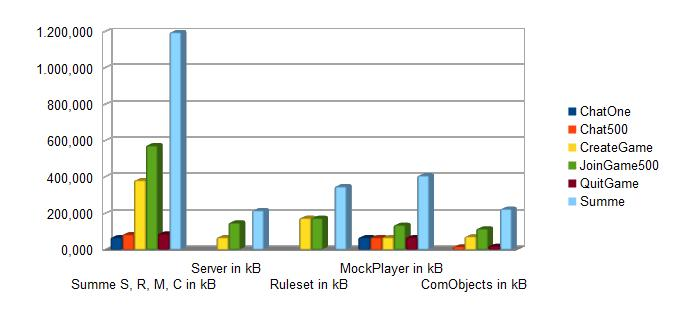
\includegraphics[scale=0.75]{1}
\end{center}
Bei ChatOne, ChatX und QuitGame gibt es kein Ruleset, da kein Spiel erstellt wird. \\
Der Speicherplatz für MockPlayer ist immer gleich, außer bei joinGame, da es noch einmal soviele Gamemaster für die Spiele gibt. \\
Der Server Speicher ist bei Create und Join Game höher da viele GameServerRepräsentations an die Spieler verschickt werden. \\
\ \\
\ \\

\noindent
\begin{tabular}{|l|r|r|r|r|r|r|}
\hline
Lobby1000Spieler & \multicolumn{1}{l|}{ChatOne} & \multicolumn{1}{l|}{Chat1000} & \multicolumn{1}{l|}{CreateGame} & \multicolumn{1}{l|}{JoinGame1000} & \multicolumn{1}{l|}{QuitGame} & \multicolumn{1}{l|}{Summe} \\ \hline
Durchschnittszeit in s & 0,052 & 0,226 & 0,191 & 0,601 & 0,104 & 1,173 \\ \hline
Gesamtspeicher in kB & 18.279,667 & 34.865,000 & 40.458,667 & 59.965,333 & 26.502,000 & 180.070,667 \\ \hline
Summe S, R, M, C in kB & 136,080 & 168,048 & 762,000 & 1.076,000 & 176,048 & 2.318,176 \\ \hline
Server in kB & 0,048 & 0,048 & 136,000 & 226,000 & 0,048 & 362,144 \\ \hline
Ruleset in kB & 0,000 & 0,000 & 346,000 & 346,000 & 0,000 & 692,000 \\ \hline
MockPlayer in kB & 136,000 & 136,000 & 136,000 & 272,000 & 136,000 & 816,000 \\ \hline
ComObjects in kB & 0,032 & 32,000 & 144,000 & 232,000 & 40,000 & 448,032 \\ \hline
\end{tabular}
\ \\
\begin{center}
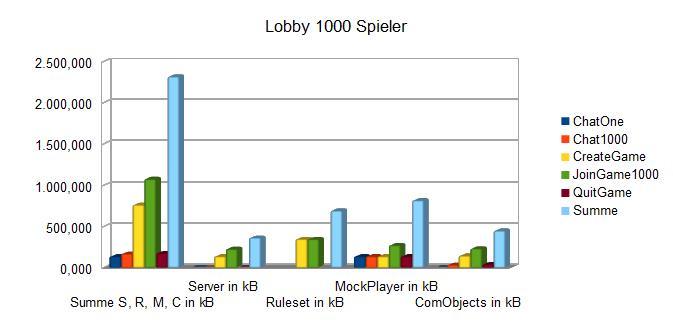
\includegraphics[scale=0.75]{2}
\end{center}
Bei ChatOne, ChatX und QuitGame gibt es kein Ruleset, da kein Spiel erstellt wird. \\
Der Speicherplatz für MockPlayer ist immer gleich, außer bei joinGame, da es noch einmal soviele Gamemaster für die Spiele gibt. \\
Der Server Speicher ist bei Create und Join Game höher da viele GameServerRepräsentations an die Spieler verschickt werden. \\
\ \\
\ \\

\noindent
\begin{tabular}{|l|r|r|r|r|r|r|}
\hline
Lobby2000Spieler & \multicolumn{1}{l|}{ChatOne} & \multicolumn{1}{l|}{Chat2000} & \multicolumn{1}{l|}{CreateGame} & \multicolumn{1}{l|}{JoinGame2000} & \multicolumn{1}{l|}{QuitGame} & \multicolumn{1}{l|}{Summe} \\ \hline
Durchschnittszeit in s & 0,038 & 0,610 & 0,577 & 2,520 & 0,117 & 3,861 \\ \hline
Gesamtspeicher in kB & 18.932,000 & 46.328,667 & 77.498,333 & 131.333,333 & 32.925,333 & 307.017,667 \\ \hline
Summe S, R, M, C in kB & 272,080 & 336,048 & 1.520,000 & 2.273,000 & 352,048 & 4.753,176 \\ \hline
Server in kB & 0,048 & 0,048 & 272,000 & 577,000 & 0,048 & 849,144 \\ \hline
Ruleset in kB & 0,000 & 0,000 & 688,000 & 688,000 & 0,000 & 1.376,000 \\ \hline
MockPlayer in kB & 272,000 & 272,000 & 272,000 & 544,000 & 272,000 & 1.632,000 \\ \hline
ComObjects in kB & 0,032 & 64,000 & 288,000 & 464,000 & 80,000 & 896,032 \\ \hline
\end{tabular}
\ \\
\begin{center}
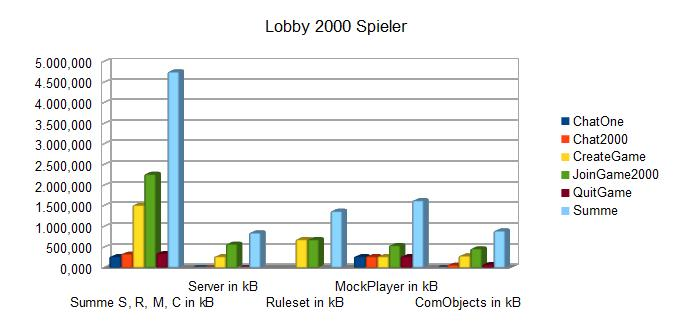
\includegraphics[scale=0.75]{3}
\end{center}
Bei ChatOne, ChatX und QuitGame gibt es kein Ruleset, da kein Spiel erstellt wird. \\
Der Speicherplatz für MockPlayer ist immer gleich, außer bei joinGame, da es noch einmal soviele Gamemaster für die Spiele gibt. \\
Der Server Speicher ist bei Create und Join Game höher da viele GameServerRepräsentations an die Spieler verschickt werden. \\

\subsubsection{Zusammenfassung}

\begin{center}
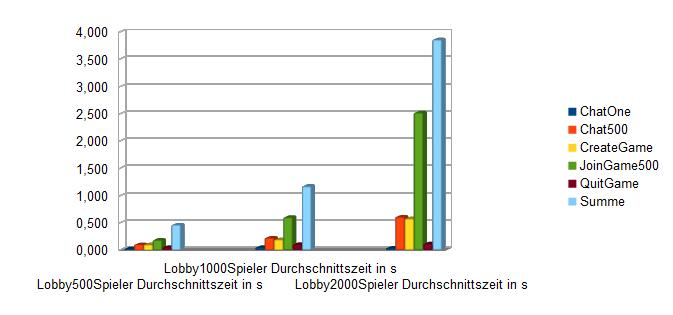
\includegraphics[scale=0.75]{7}
\end{center}

\begin{center}
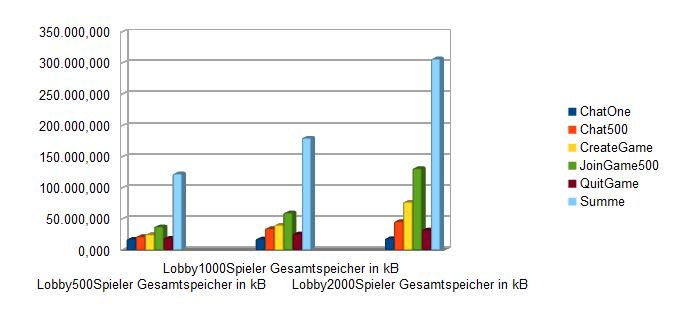
\includegraphics[scale=0.75]{8}
\end{center}

JoinGame braucht die meiste Zeit und Gesamtspeicher, da vorher noch die entsprechende Zahl an Spielen erstellt werden muss.


\subsection{Server}

\noindent
\begin{tabular}{|l|r|r|r|r|r|r|}
\hline
GameServer100 & \multicolumn{1}{l|}{ChatOne} & \multicolumn{1}{l|}{Chat300} & \multicolumn{1}{l|}{KickPlayer} & \multicolumn{1}{l|}{GameMasterLeave} & \multicolumn{1}{l|}{StartGame} & \multicolumn{1}{l|}{Summe} \\ \hline
Durchschnittszeit in s & 0,126 & 0,158 & 0,169 & 0,191 & 0,169 & 0,812 \\ \hline
Gesamtspeicher in kB & 20.341,000 & 21.002,333 & 21.290,000 & 23.180,667 & 20.965,000 & 106.779,000 \\ \hline
Summe S, R, M, C in kB & 163,792 & 170,192 & 586,256 & 794,656 & 304,576 & 2.019,472 \\ \hline
Server in kB & 45,656 & 45,656 & 453,000 & 655,000 & 49,656 & 1.248,968 \\ \hline
Ruleset in kB & 37,336 & 37,336 & 37,336 & 37,336 & 155,000 & 304,344 \\ \hline
MockPlayer in kB & 40,800 & 40,800 & 40,800 & 40,800 & 40,800 & 204,000 \\ \hline
ComObjects in kB & 40,000 & 46,400 & 55,120 & 61,520 & 59,120 & 262,160 \\ \hline
\end{tabular}
\ \\
\begin{center}
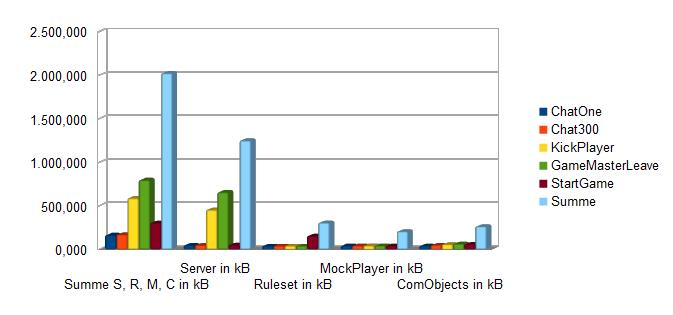
\includegraphics[scale=0.75]{4}
\end{center}
Der Server Speicher ist bei KickPlayer und GameMasterLeave sehr viel höher, da viele GameServerRepräsentations an die Spieler verschickt werden. \\
Das Ruleset ist bei StartGame am höchsten, da es das Spiel startet und Karten etc. verschickt.

\ \\
\ \\

\noindent
\begin{tabular}{|l|r|r|r|r|r|r|}
\hline
GameServer250 & \multicolumn{1}{l|}{ChatOne} & \multicolumn{1}{l|}{Chat750} & \multicolumn{1}{l|}{KickPlayer} & \multicolumn{1}{l|}{GameMasterLeave} & \multicolumn{1}{l|}{StartGame} & \multicolumn{1}{l|}{Summe} \\ \hline
Durchschnittszeit in s & 0,225 & 0,291 & 0,315 & 0,419 & 0,252 & 1,503 \\ \hline
Gesamtspeicher in kB & 31.476,333 & 34.668,000 & 42.475,333 & 53.536,667 & 31.783,667 & 193.940,000 \\ \hline
Summe S, R, M, C in kB & 404,936 & 420,936 & 2.962,936 & 4.148,936 & 755,000 & 8.692,744 \\ \hline
Server in kB & 114,000 & 114,000 & 2.634,000 & 3.820,000 & 124,000 & 6.806,000 \\ \hline
Ruleset in kB & 88,936 & 88,936 & 88,936 & 88,936 & 384,000 & 739,744 \\ \hline
MockPlayer in kB & 102,000 & 102,000 & 102,000 & 102,000 & 102,000 & 510,000 \\ \hline
ComObjects in kB & 100,000 & 116,000 & 138,000 & 138,000 & 145,000 & 637,000 \\ \hline
\end{tabular}
\ \\
\begin{center}
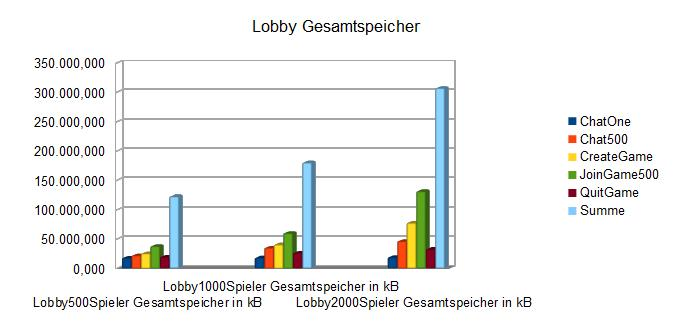
\includegraphics[scale=0.75]{5}
\end{center}
Der Server Speicher ist bei KickPlayer und GameMasterLeave sehr viel höher, da viele GameServerRepräsentations an die Spieler verschickt werden. \\
Das Ruleset ist bei StartGame am höchsten, da es das Spiel startet und Karten etc. verschickt.
\ \\
\ \\

\noindent
\begin{tabular}{|l|r|r|r|r|r|r|}
\hline
GameServer500 & \multicolumn{1}{l|}{ChatOne} & \multicolumn{1}{l|}{Chat1500} & \multicolumn{1}{l|}{KickPlayer} & \multicolumn{1}{l|}{GameMasterLeave} & \multicolumn{1}{l|}{StartGame} & \multicolumn{1}{l|}{Summe} \\ \hline
Durchschnittszeit in s & 0,485 & 0,583 & 0,620 & 1,011 & 0,501 & 3,199 \\ \hline
Gesamtspeicher in kB & 42.339,000 & 45.215,667 & 74.373,333 & 91.421,667 & 45.612,333 & 298.962,000 \\ \hline
Summe S, R, M, C in kB & 806,000 & 838,000 & 10.801,000 & 15.844,000 & 1.590,000 & 29.879,000 \\ \hline
Server in kB & 228,000 & 228,000 & 10.147,000 & 15.158,000 & 248,000 & 26.009,000 \\ \hline
Ruleset in kB & 174,000 & 174,000 & 174,000 & 174,000 & 846,000 & 1.542,000 \\ \hline
MockPlayer in kB & 204,000 & 204,000 & 204,000 & 204,000 & 204,000 & 1.020,000 \\ \hline
ComObjects in kB & 200,000 & 232,000 & 276,000 & 308,000 & 292,000 & 1.308,000 \\ \hline
\end{tabular}
\ \\
\begin{center}
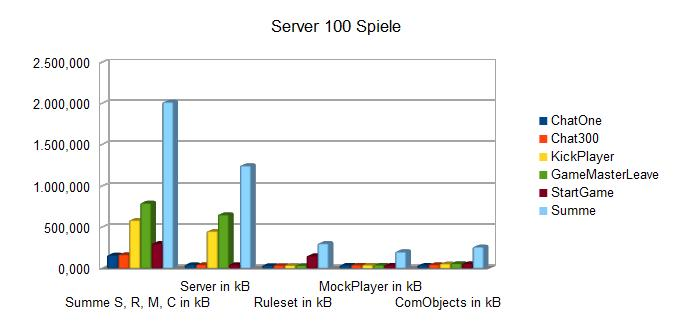
\includegraphics[scale=0.75]{6}
\end{center}
Der Server Speicher ist bei KickPlayer und GameMasterLeave sehr viel höher, da viele GameServerRepräsentations an die Spieler verschickt werden. \\
Das Ruleset ist bei StartGame am höchsten, da es das Spiel startet und Karten etc. verschickt.

\subsubsection{Zusammenfassung}

\begin{center}
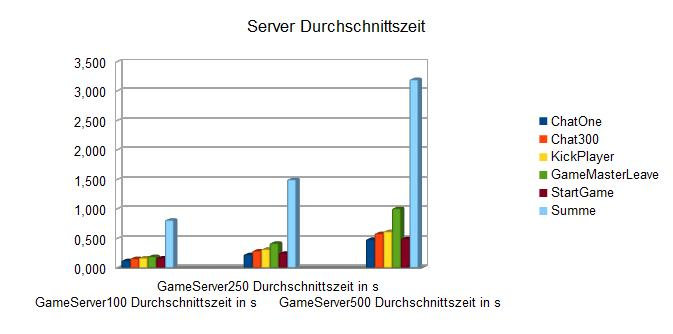
\includegraphics[scale=0.75]{9}
\end{center}
Bei vielen Spielern verbraucht der Server exponentiell viel mehr Speicher, da sehr viele GameServerUpdates an alle Spieler verschickt verden und diese viel Speicher brauchen.

\begin{center}
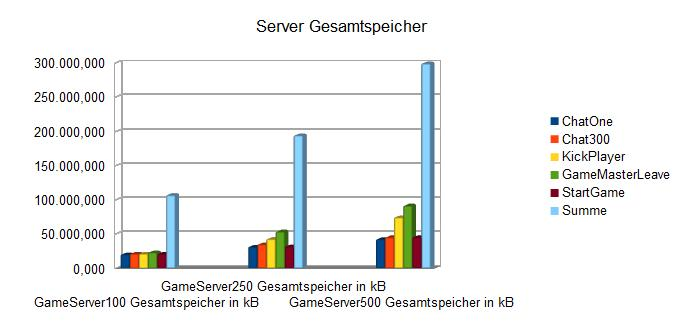
\includegraphics[scale=0.75]{10}
\end{center}
GameMasterLeave braucht die meiste Zeit und Gesamtspeicher, da alle Spieler die GameLobby verlassen und entsprechende Updates verschickt werden müssen


\section{Weitere Tests}
	\subsection{BETA-Test}
	Es wurde ein BETA-Test über ein Wochenende gestartet. Es nahmen 15 unabhängige Personen daran teil.
	Jede Anmerkung wurde ausgewertet und nach Möglichkeit verbessert oder umgesetzt.
	\begin{itemize}
	\item Doppelter Name: Es bestand die Möglichkeit sich mit dem Namen 'TestSpieler' einzuloggen und zusätzlich nocheinmal 		mit dem Namen 'Testspieler '. Die doppelte Nutzung eines Namens durch Anfügen von Leerzeichen wurde unterbunden.
	\item Handbuch: Die Erklärung zum Serverstart ist nicht ausreichend genug. Das Kapitel Installation wurde deshalb 			überarbeitet.
	\item Rundenanzahl: Es wurde angemerkt, dass die Anzeige einer Rundenzahl sinnvoll wäre, sodass man sehen kann in 			welcher man sich befindet, ohne mitzuzählen. Die Rundenzahl wird nun zusätzlich im Infofenster angezeigt, in dem der			Spieler auch seine anderen Informationen sehen kann.
	\item Beschränkte Länge des Namens: Da die Länge des Spielernamens zuvor nicht eingeschränkt war, und deshalb nicht 		der ganze Name im Spielfenster dargestellt werden konnte, wurde eine Begrenzung der Länge eingeführt.
	\end{itemize}

\end{document}